\chapter{Detection methods} \label{chap:detection_methods}

%versions of the detector
\section{Scintillation}

This section summarizes some key aspects for our use case scenario taken from Chapter 8 of Ref. \cite{knoll2010radiation}, where an in depth exploration of various scintillating materials and their properties is presented. LYSO:Ce belongs to the family of inorganic scintillating materials, while plastic scintillators belong to the organic family. Scintillation in general arises from the de-excitation of electrons in higher energy states inside the material, inorganic scintillators however, have only discrete energy states to jump between. The lower energy state is known as the Valence band and represents the energy of those electrons which are bound to the crystal lattice, the conduction band on the other hand, is the upper electron energy level in which they are free to travel across the crystal. Energy absorption inside the crystal therefore occurs when an electron is promoted across the band gap towards the conduction band, de-excitation of these electrons back into the valence band is not very common, and the photons emitted from this transition are often highly energetic, leaving them outside the visible range.

\begin{figure}[H]
    \centering
    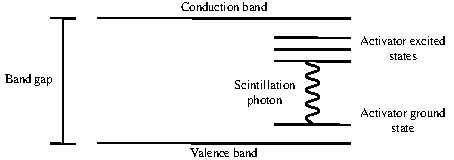
\includegraphics[width=0.7\textwidth]{detection_methods/Scintillation.pdf}
    \caption{Electronic energy level structure in activated inorganic scintillators, adapted from \cite[Ch.~8]{knoll2010radiation}.}
    \label{fig:Scintillation}
\end{figure}

In order to increase the production of optical photons and probability of de-excitation to lower energy states, some inorganic crystals are activated with small amounts of other elements, these activators induce energy states in between the band gap at specific places in the crystal lattice, creating new channels through which the electrons can fall back into the valence band. In our case LYSO:Ce, therefore represents a Cerium-activated LYSO crystal. Cerium in particular possesses a short decay time, between 20 and 80 ns, making the crystal faster than some inorganics but also slow compared to organic scintillators with decay times of just a few nanoseconds.

\section{PMTs}

Photomultipliers are very useful tools in particle detection. Since some detection methods rely on the measurement of photons it is very important to make use of every single one. Some PMs are capable of creating measurable electrical signals from single photon interactions, provoking an electron avalanche that can be easily read with various devices. Photomultiplier Tubes are the most common light amplifiers paired with scintillators, they are however bulky and require very high voltages to operate. An in-depth description of this and other types of Photomultipliers can be found in Ref. \cite{knoll2010radiation} Chap. 9.

\section{SiPM advantages}

CosmicWatch is meant to be a portable, easy-to-build, and economical device, making PMTs not suitable for the overall intention of the project. This, however, is fully solved by Silicon Photomultipliers, their small form factor, relatively low operating voltage, and good efficiency at wavelengths near the emission maxima of common scintillating materials, turn them into an ideal candidate for use in this project. For further details on SiPMs also read Ref. \cite{knoll2010radiation} Chap. 9 and Ref. \cite{Onsemi_SiPM_intro}.

A Silicon Photomultiplier is an array of Geiger-mode avalanche-photodiodes. To make this more digestible we can introduce these concepts one by one. A photodiode is essentially made of a P-N semiconductor junction, where scintillation photons can create new electron-hole pairs that will be accelerated by the bias voltage applied to the diode. However, this process alone produces small signals, making a preamplification stage necessary. Avalanche photodiodes alleviate this problem by increasing the bias voltage, therefore giving the photoelectrons higher energies, allowing them to collide and produce new electron-hole pairs that will also be detected. When the bias voltage rises sufficiently high, the regions where photoelectrons multiply merge together, making one big avalanche, this is the so-called Geiger mode of APDs, and this high voltage receives the name of Breakdown Voltage. Geiger mode APDs can produce a large output from a single scintillation photon. The difference Between Bias and Breakdown Voltage is known as Over-voltage.

SiPMs however, also have some disadvantages, since they are based on the transport of photoelectrons, the output can vary with temperature, as high temperatures can create electron-hole pairs that will be read as a photon interaction. These events are called dark pulses and represent a random noise in the signal.

The SiPM used and tested throughout this work is a MicroFJ-300XX-TSV by Onsemi \cite{Onsemi_SiPM} (Fig. \ref{fig:Onsemi_SiPM}), which has an active area of $3.07 \times 3.07$ \unit{\mm\squared} and a microcell size of 35 \unit{\micro\m}. In this case, the operating voltage ranges between 25.2 and 30.7 \unit{\V}, which can be obtained using a DC to DC booster (see Section \ref{sec:DC_DC}), no longer requiring the high voltages of PMTs. We are currently operating at a Breakdown Voltage of around 24 V and an Over-voltage of 4 V, which according to Ref. \cite{Onsemi_SiPM} produces a relatively high dark count rate (50-150 \unit{\kilo\Hz\per\mm\squared} at 21 $^\circ$C), potentially affecting energy resolution.

\begin{figure}[H]
    \centering
    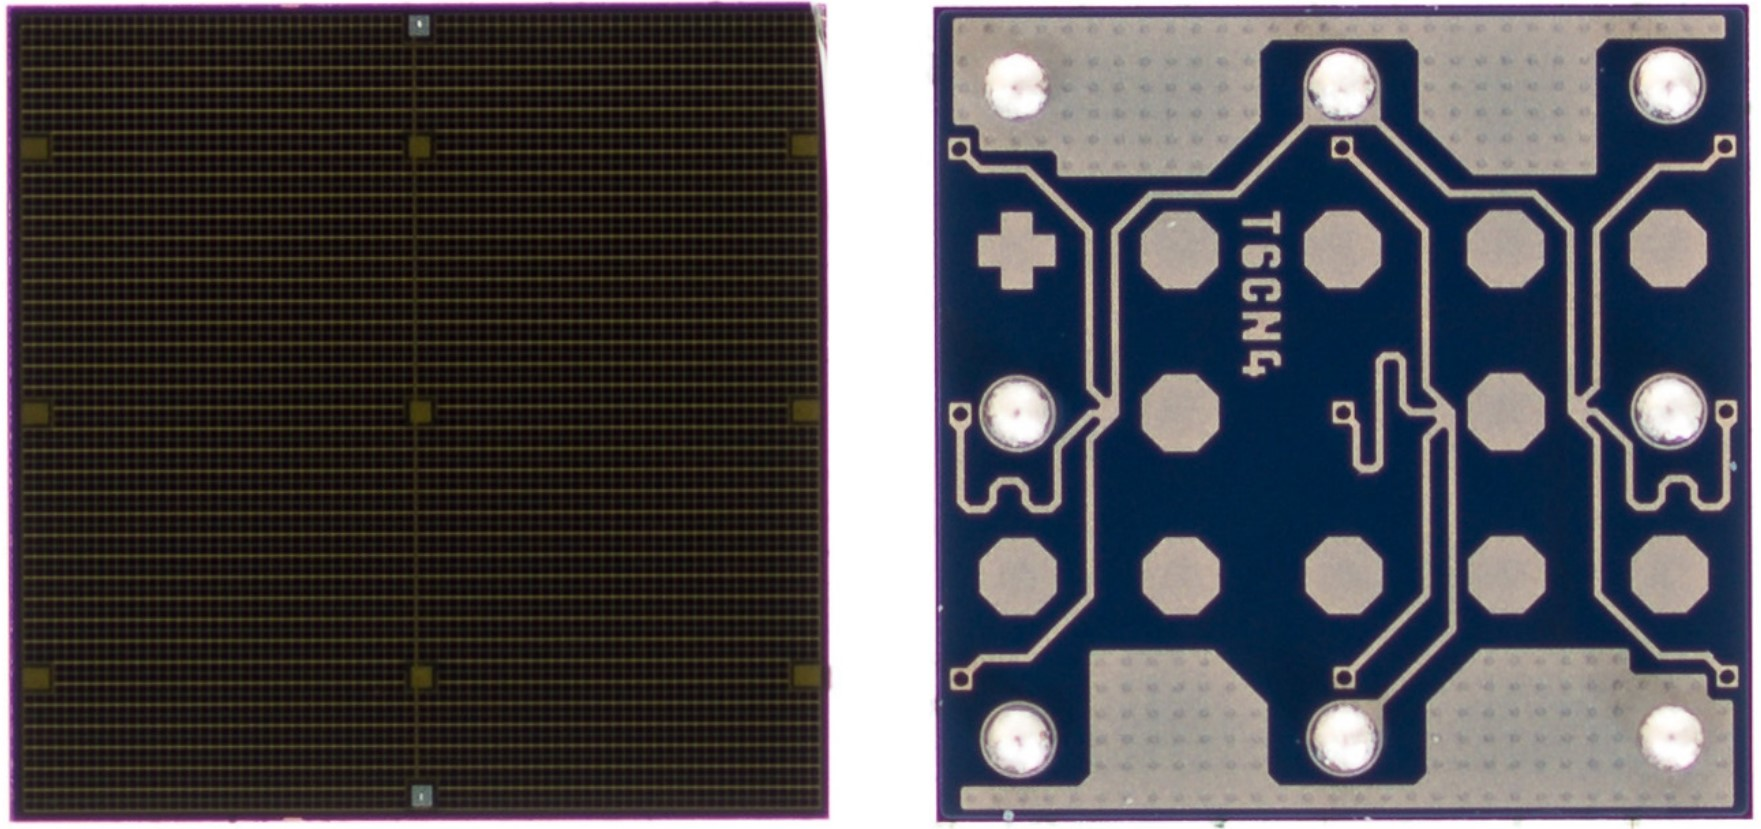
\includegraphics[width=0.8\textwidth]{detection_methods/MicroFJ−300XX−TSV.jpeg}
    \caption{Onsemi MicroFJ-300XX-TSV. Taken from \cite{Onsemi_SiPM}.}
    \label{fig:Onsemi_SiPM}
\end{figure}